%%%%%%%%%%%%%%%%%%%%%%%%%%%%%%%%%%%%%%%%%%%%%%%%%%%%%%%%%%%%%%%
%
% Welcome to Overleaf --- just edit your LaTeX on the left,
% and we'll compile it for you on the right. If you open the
% 'Share' menu, you can invite other users to edit at the same
% time. See www.overleaf.com/learn for more info. Enjoy!
%
%%%%%%%%%%%%%%%%%%%%%%%%%%%%%%%%%%%%%%%%%%%%%%%%%%%%%%%%%%%%%%%


% Inbuilt themes in beamer
\documentclass{beamer}

% Theme choice:
\usetheme{CambridgeUS}

% Title page details: 
\title{Assignment 5} 
\author{Varun Gupta \\ cs21btech11060}
\date{\today}
\logo{\large \LaTeX{}}


\begin{document}

% Title page frame
\begin{frame}
    \titlepage 
\end{frame}

% Remove logo from the next slides
\logo{}


% Outline frame
\begin{frame}{Outline}
    \tableofcontents
\end{frame}

\section{Class 12 Solutions}
\begin{frame}{Exercise 13.2}
    \begin{block}{Q.10}
        Events A and B are such that $P(A) = \frac{1}{2}, P(B) = \frac{7}{12}$ and $P(\overline{A}) \cup P(\overline{B}) = \frac{1}{4}$. State whether A and B are independent?
    \end{block}
    \begin{block}{Solution:}
        For two events to be independent, We know
        \begin{equation}
            P(A) \cdot P(B) = P(A \cap B)
        \end{equation}
        Also,
        \begin{equation}
            P(\overline{A}) \cup P(\overline{B}) = \overline{P(A \cap B)} = \frac{1}{4}
        \end{equation}
        \begin{equation}
            \Rightarrow P(A \cap B) = 1-\frac{1}{4} = \frac{3}{4}
        \end{equation}
    \end{block}
\end{frame}
\begin{frame}
        But,
        \begin{equation}
            P(A) \cdot P(B) = \frac{1}{2} \times \frac{7}{12} = \frac{7}{24}
        \end{equation}
        Hence, A \& B are not independent events.
        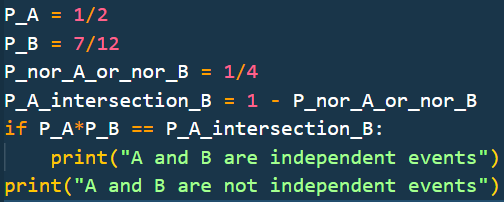
\includegraphics{figures/fig.png}
\end{frame}
\end{document}